\documentclass{article}

\usepackage[german]{babel}

% Set page size and margins
% Replace `letterpaper' with `a4paper' for UK/EU standard size
\usepackage[letterpaper,top=2cm,bottom=2cm,left=3cm,right=3cm,marginparwidth=1.75cm]{geometry}

% Useful packages
\usepackage{listings}
\usepackage{xcolor}
\usepackage{amsmath}
\usepackage{graphicx}
\usepackage[colorlinks=true, allcolors=blue]{hyperref}
\usepackage[colorinlistoftodos]{todonotes}

\definecolor{codegray}{rgb}{0.5,0.5,0.5}
\definecolor{backcolour}{rgb}{0.97,0.97,0.97}
\definecolor{yellouw}{rgb}{0.62,0.53334,0.050}
\definecolor{keywordcolor}{rgb}{0.0, 0.33, 0.84}  % Blauton für Keywords
\definecolor{stringcolor}{rgb}{0.2, 0.7, 0.2}  % Grünton für Strings
\definecolor{commentcolor}{rgb}{0.5, 0.5, 0.5}  % Grauton für Kommentare
\newcommand{\CodeSymbol}[1]{\textcolor{red}{#1}}
\definecolor{pred}{rgb}{0.9,0.3,0.3}

\lstdefinestyle{codeStyle}{
    backgroundcolor=\color{backcolour},
    numberstyle=\tiny\color{codegray},
     basicstyle=\ttfamily\footnotesize,
    columns=fullflexible,
    framexleftmargin=15pt,
    texcl=true,
    breakatwhitespace=false,
    breaklines=true,
    captionpos=b,
    keepspaces=true,
    numbers=left,
    numbersep=10pt,
    showspaces=false,
    showstringspaces=false,
    showtabs=false,
    literate={\{}{{\CodeSymbol{\{}}}1
                  {\}}{{\CodeSymbol{\}}}}1
                  {>}{{\CodeSymbol{$>$}}}1
                  {\.}{{\CodeSymbol{.}}}1
                  {;}{{\CodeSymbol{$;$}}}1,
    moredelim=[il][\textcolor{yellouw}@\textcolor{yellouw}]{@},
    tabsize=2,
    keywordstyle=\color{keywordcolor}\bfseries,  % Stil für Keywords
    stringstyle=\color{pred},  % Stil für Strings
    commentstyle=\color{stringcolor}\itshape,  % Stil für Kommentare
    morekeywords={abstract, continue, for, new, switch, assert, default, goto, package,
    synchronized, boolean, do, if, private, this, break, double, implements,
    protected, throw, byte, else, import, public, throws, case, enum,
    instanceof, return, transient, catch, extends, int, short, try, char,
    final, interface, static, void, class, finally, long, strictfp, volatile,
    const, float, native, super, while, var},  % Erweiterte Keyword-Liste
}
% TODO: header
\title{Programmentwurf – Protokoll}

\begin{document}


\begin{titlepage}
\begin{center}
\vspace*{-2cm}
\hfill
\includegraphics[width=4cm]{dhbw-logo.png}\\[2cm]
{\Huge Advanced Software Engineering}\\[1cm]
{\Huge\scshape Programmentwurf - Protokoll}\\[1cm]
{\large von}\\[0.5cm]
\todo{Namen + Matrikelnummern einfügen}
{\large\bfseries Vorname Nachname (123456)}\\[0.5cm]
{\large\bfseries Vorname Nachname (123456)}\\[0.5cm]
{\large\bfseries Vorname Nachname (123456)}\\[1.5cm]

{\large Abgabedatum 04. Mai 2025}
\vfill
\end{center}
\end{titlepage}

\definecolor{sickblue}{RGB}{52, 101, 204}
\newcommand{\task}[1]{\textit{\textcolor{sickblue}{[#1]}\newline\newline}}

{
  \hypersetup{linkcolor=black}
  \tableofcontents
}
\section{SOLID (8P)}

\subsection{Analyse SRP (3P)}
\task{jeweils eine Klasse als positives und negatives Beispiel für SRP; jeweils UML und Beschreibung der Aufgabe bzw. der Aufgaben und möglicher Lösungsweg des Negativ-Beispiels (inkl. UML)}

\subsubsection*{Positiv-Beispiel}
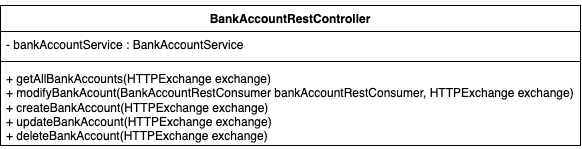
\includegraphics[width=\linewidth]{kapitel3_solid/BankAccountRestController.png}
Der BankAccountRestController ist eine Klasse, welche die CRUD-Endpunkte für die Bankkonten anbietet.

\subsubsection*{Negativ-Beispiel}
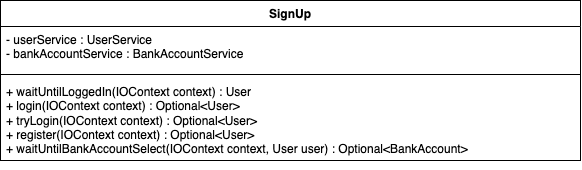
\includegraphics[width=\linewidth]{kapitel3_solid/SignUp.png}
Die SingUp-Klasse ist für das Anmelden und Registrieren eines Benutzers vor dem Programm dar. Dadurch das die Methoden waitUntilLoggedIn() sowie waitUntilBankAccountIsSelect() eher weniger mit dem Anmelden zu tun haben, müsste man diese in eine neue Klasse wie zum Beispiel WaitUntil extrahieren.



\subsection{Analyse OCP (3P)}
\task{jeweils eine Klasse als positives und negatives Beispiel für OCP;  jeweils UML und Analyse mit Begründung, warum das OCP erfüllt/nicht erfüllt wurde – falls erfüllt: warum hier sinnvoll/welches Problem gab es? Falls nicht erfüllt: wie könnte man es lösen (inkl. UML)?}

\subsubsection*{Positiv-Beispiel}
Die Klasse \texttt{HTMLTag} wurde im Projekt als Interface definiert, das eine einheitliche Methode \texttt{build()} bereitstellt. Alle HTML-Komponenten (wie \texttt{HTMLTableRow}, \texttt{HTMLDataCell} oder \texttt{HTMLHeaderCell}) implementieren dieses Interface. Dadurch können neue HTML-Elemente flexibel ergänzt werden, ohne die bestehende Logik anzupassen.
\newline
Beispielsweise kann der \texttt{FinanceReportBuilder} über eine Liste von HTMLTag-Elementen iterieren und sie per \texttt{build()} zu HTML umwandeln. Dies ist dabei unabhängig von der konkreten Implementierung.
\newline
Dieses Design erfüllt das Open/Closed Principle, da die Funktionalität durch neue Klassen erweitert, aber das bestehende Interface und die Verarbeitung nicht verändert werden müssen.
\newline
\textbf{Warum hier sinnvoll?} Das HTML-Reporting soll flexibel auf neue Anforderungen reagieren können (z.B. neue Zeilentypen oder Zellenformate). Mit dem Interface-Ansatz kann dies erfolgen, ohne dass zentrale Komponenten wie der \texttt{ReportBuilder} angepasst werden müssen.
\newline\newline
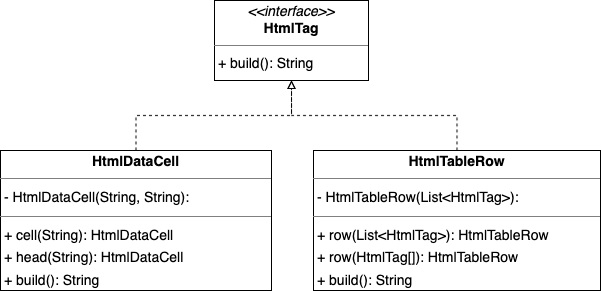
\includegraphics[width=\linewidth]{kapitel3_solid/positive_ocp.png}

\subsubsection*{Negativ Beispiel}
Die Klasse \texttt{Localization} ist für die Übersetzung von Texten in verschiedene Sprachen zuständig. Sie verwendet intern \texttt{ResourceBundle}, um Übersetzungen aus \texttt{.properties}-Dateien basierend auf einem Sprachcode zu laden (\texttt{messages\_en.properties}, \texttt{messages\_de.properties})
\newline\newline
\textbf{Warum wird das OCP hier verletzt?}\newline
Die Klasse ist nicht offen für Erweiterungen, sondern muss bei jeder neuen Anforderung direkt geändert werden. Dadurch verstößt sie gegen das Open/Closed Principle:
\begin{itemize}
    \item Neue Sprachen (z.B. „fr“) müssen im Code zur Liste \texttt{supportedLanguages} hinzugefügt werden.
    \item Neue Übersetzungsquellen (z.B. JSON-Dateien, Datenbank, REST-API) erfordern Änderungen an der Methode \texttt{setLocale(...)}, da dort \texttt{ResourceBundle} fest eingebunden ist.
    \item Eine dynamische Erweiterung oder das Nachladen von Übersetzungen zur Laufzeit ist nicht möglich, ohne die bestehende Klasse zu verändern.
\end{itemize}
\newline
\textbf{Lösungsansatz:}\newline
Um das Open/Closed Principle einzuhalten, sollte die eigentliche Übersetzungslogik in ein Interface ausgelagert werden, z.B. \texttt{TranslationProvider}. Damit könnten unterschiedliche Implementierungen genutzt werden, ohne \texttt{Localization} ändern zu müssen:
\newline
\lstinputlisting[language=Java,style=codeStyle]{kapitel3_solid/translationProvider.java}
Die Localization-Klasse müsste dann nur noch ein solches Interface nutzen – und wäre offen für Erweiterung, aber geschlossen für Modifikation. Beispielhafte Implementierungen könnten dann die folgenden sein: \newline
\begin{itemize}
    \item ResourceBundleTranslationProvider
    \item JsonTranslationProvider
    \item ApiTranslationProvider
\end{itemize}
\subsubsection*{UML-Vergleich}
\textbf{Ist-Zustand:}
\begin{figure}[htbp]
    \centering
    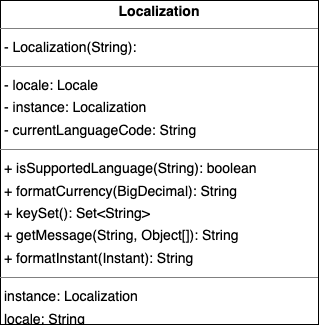
\includegraphics[width=0.5\linewidth]{kapitel3_solid/negative_ocp_ist.drawio.png}
\end{figure}
\newline
\textbf{Nachher:}
\begin{figure}[htbp]
    \centering
    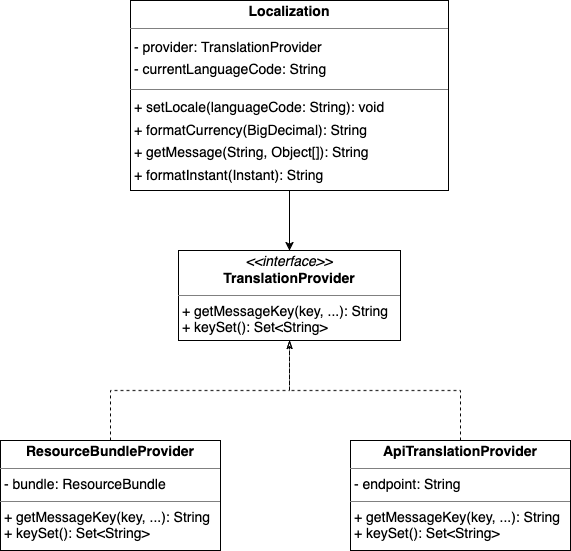
\includegraphics[width=0.65\linewidth]{kapitel3_solid/negative_ocp_neu.drawio.png}
\end{figure}


\subsection{Analyse [LSP/ISP/DIP] (2P)}
\task{jeweils eine Klasse als positives und negatives Beispiel für entweder LSP oder ISP oder DIP;  jeweils UML und Begründung, warum hier das Prinzip erfüllt/nicht erfüllt wird; beim Negativ-Beispiel UML einer möglichen Lösung hinzufügen}
\task{Anm.: es darf nur ein Prinzip ausgewählt werden; es darf NICHT z.B. ein positives Beispiel für LSP und ein negatives Beispiel für ISP genommen werden}
\\
\textbf{Gewähltes Prinzip: ISP}

\subsubsection*{Positiv-Beispiel}
Die Schnittstelle \texttt{BankAccountService} definiert ausschließlich Methoden rund um Bankkonten und hat somit eine sehr saubere Trennung: Die Schnittstelle ist spezifisch und auf eine einzige Domäne fokussiert.
\lstinputlisting[language=Java,style=codeStyle]{kapitel3_solid/ISP_BankAccountService.java}
\textbf{Begründung}
\begin{itemize}
    \item Interface ist spezialisiert und damit gut für Testbarkeit und Wartung
    \item Folgeprinzip: niedrige Kopplung, hohe Kohäsion
\end{itemize}
\textbf{UML}
\begin{figure}[htbp]
    \centering
    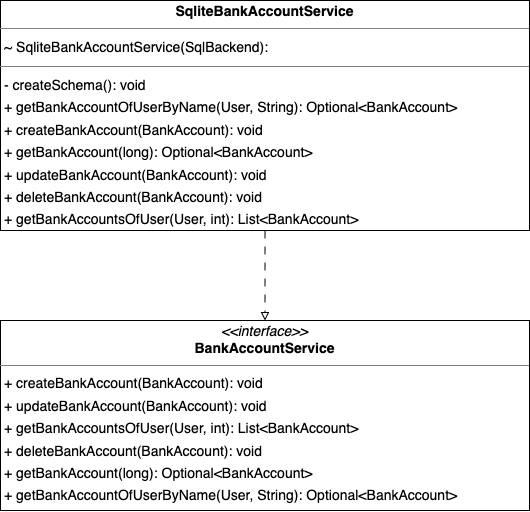
\includegraphics[width=0.65\linewidth]{kapitel3_solid/ISP_pos_bankaccount.drawio.png}
\end{figure}

\subsubsection*{Negativ-Beispiel}
Das Command-Interface wird von allen Befehlen im Terminal verwendet und sieht so aus:
\lstinputlisting[language=Java,style=codeStyle]{kapitel3_solid/ISP_Command.java}
Das wirkt erstmal schlank, aber: In der Praxis gibt es viele Commands, die keine Argumente brauchen, oder deren Verwendung durch das Interface erzwungen wird, obwohl sie sie gar nicht nutzen.
\textbf{Begründung}
\begin{itemize}
    \item Ein Interface sollte nur das vorschreiben, was für den jeweiligen Fall zwingend nötig ist.
    \item \texttt{Command} ist zu allgemein – spezialisierte Commands (z.B. Info-Commands vs. System-Commands) sollten getrennte Interfaces bekommen.
    \item Verstöße gegen ISP führen oft zu optionalen, leeren oder irrelevanten Implementierungen → das ist ein Code-Smell.
\end{itemize}
\textbf{UML - Ist-Zustand}\newline
\begin{figure}[htbp]
    \centering
    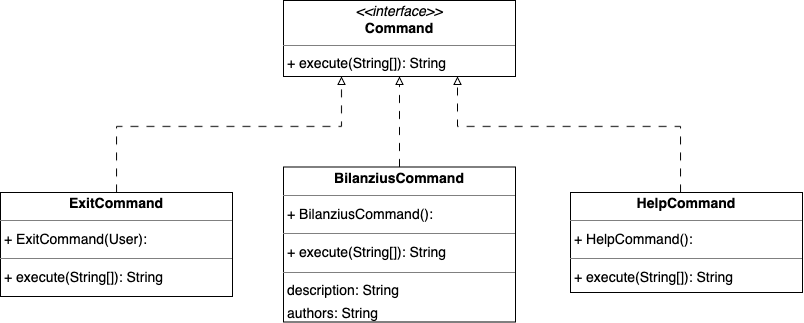
\includegraphics[width=\linewidth]{kapitel3_solid/ISP_neg_Command2.drawio.png}
\end{figure}
\newline
\textbf{Verbesserungsvorschlag}\newline
Trennen von \texttt{Command} in spezifischere Interfaces, z.B.:
\lstinputlisting[language=Java,style=codeStyle]{kapitel3_solid/ISP_Commands.java}
Dann können z.B. \texttt{HelpCommand} und \texttt{ExitCommand} \texttt{SimpleCommand} implementieren, während z.B. ein \textbf{CreateCategoryCommand} ein ArgumentCommand implementiert.\newline\newline
\textbf{UML Verbesserung}
\begin{figure}[htbp]
    \centering
    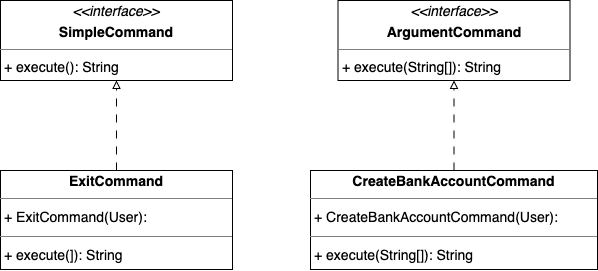
\includegraphics[width=\linewidth]{kapitel3_solid/ISP_neg_betterCommand2.drawio.png}
\end{figure}
\section{SOLID (8P)}

\subsection{Analyse SRP (3P)}
\task{jeweils eine Klasse als positives und negatives Beispiel für SRP; jeweils UML und Beschreibung der Aufgabe bzw. der Aufgaben und möglicher Lösungsweg des Negativ-Beispiels (inkl. UML)}

\subsubsection*{Positiv-Beispiel}
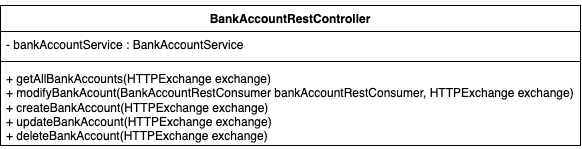
\includegraphics[width=\linewidth]{kapitel3_solid/BankAccountRestController.png}
Der BankAccountRestController ist eine Klasse, welche die CRUD-Endpunkte für die Bankkonten anbietet.

\subsubsection*{Negativ-Beispiel}
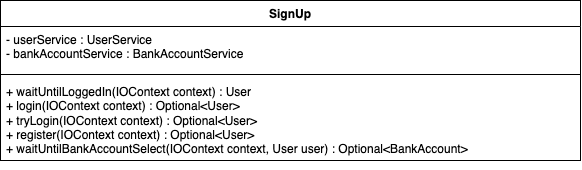
\includegraphics[width=\linewidth]{kapitel3_solid/SignUp.png}
Die SingUp-Klasse ist für das Anmelden und Registrieren eines Benutzers vor dem Programm dar. Dadurch das die Methoden waitUntilLoggedIn() sowie waitUntilBankAccountIsSelect() eher weniger mit dem Anmelden zu tun haben, müsste man diese in eine neue Klasse wie zum Beispiel WaitUntil extrahieren.



\subsection{Analyse OCP (3P)}
\task{jeweils eine Klasse als positives und negatives Beispiel für OCP;  jeweils UML und Analyse mit Begründung, warum das OCP erfüllt/nicht erfüllt wurde – falls erfüllt: warum hier sinnvoll/welches Problem gab es? Falls nicht erfüllt: wie könnte man es lösen (inkl. UML)?}

\subsubsection*{Positiv-Beispiel}
Die Klasse \texttt{HTMLTag} wurde im Projekt als Interface definiert, das eine einheitliche Methode \texttt{build()} bereitstellt. Alle HTML-Komponenten (wie \texttt{HTMLTableRow}, \texttt{HTMLDataCell} oder \texttt{HTMLHeaderCell}) implementieren dieses Interface. Dadurch können neue HTML-Elemente flexibel ergänzt werden, ohne die bestehende Logik anzupassen.
\newline
Beispielsweise kann der \texttt{FinanceReportBuilder} über eine Liste von HTMLTag-Elementen iterieren und sie per \texttt{build()} zu HTML umwandeln. Dies ist dabei unabhängig von der konkreten Implementierung.
\newline
Dieses Design erfüllt das Open/Closed Principle, da die Funktionalität durch neue Klassen erweitert, aber das bestehende Interface und die Verarbeitung nicht verändert werden müssen.
\newline
\textbf{Warum hier sinnvoll?} Das HTML-Reporting soll flexibel auf neue Anforderungen reagieren können (z.B. neue Zeilentypen oder Zellenformate). Mit dem Interface-Ansatz kann dies erfolgen, ohne dass zentrale Komponenten wie der \texttt{ReportBuilder} angepasst werden müssen.
\newline\newline
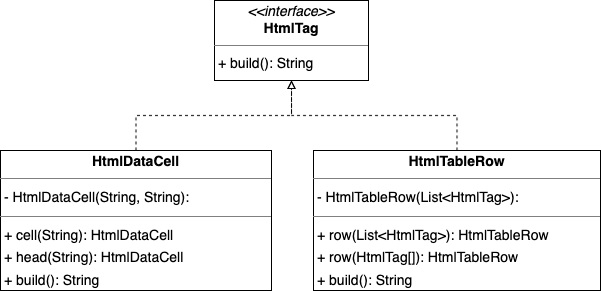
\includegraphics[width=\linewidth]{kapitel3_solid/positive_ocp.png}

\subsubsection*{Negativ Beispiel}
Die Klasse \texttt{Localization} ist für die Übersetzung von Texten in verschiedene Sprachen zuständig. Sie verwendet intern \texttt{ResourceBundle}, um Übersetzungen aus \texttt{.properties}-Dateien basierend auf einem Sprachcode zu laden (\texttt{messages\_en.properties}, \texttt{messages\_de.properties})
\newline\newline
\textbf{Warum wird das OCP hier verletzt?}\newline
Die Klasse ist nicht offen für Erweiterungen, sondern muss bei jeder neuen Anforderung direkt geändert werden. Dadurch verstößt sie gegen das Open/Closed Principle:
\begin{itemize}
    \item Neue Sprachen (z.B. „fr“) müssen im Code zur Liste \texttt{supportedLanguages} hinzugefügt werden.
    \item Neue Übersetzungsquellen (z.B. JSON-Dateien, Datenbank, REST-API) erfordern Änderungen an der Methode \texttt{setLocale(...)}, da dort \texttt{ResourceBundle} fest eingebunden ist.
    \item Eine dynamische Erweiterung oder das Nachladen von Übersetzungen zur Laufzeit ist nicht möglich, ohne die bestehende Klasse zu verändern.
\end{itemize}
\newline
\textbf{Lösungsansatz:}\newline
Um das Open/Closed Principle einzuhalten, sollte die eigentliche Übersetzungslogik in ein Interface ausgelagert werden, z.B. \texttt{TranslationProvider}. Damit könnten unterschiedliche Implementierungen genutzt werden, ohne \texttt{Localization} ändern zu müssen:
\newline
\lstinputlisting[language=Java,style=codeStyle]{kapitel3_solid/translationProvider.java}
Die Localization-Klasse müsste dann nur noch ein solches Interface nutzen – und wäre offen für Erweiterung, aber geschlossen für Modifikation. Beispielhafte Implementierungen könnten dann die folgenden sein: \newline
\begin{itemize}
    \item ResourceBundleTranslationProvider
    \item JsonTranslationProvider
    \item ApiTranslationProvider
\end{itemize}
\subsubsection*{UML-Vergleich}
\textbf{Ist-Zustand:}
\begin{figure}[htbp]
    \centering
    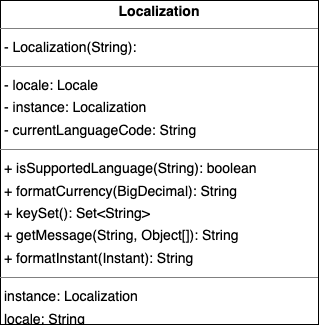
\includegraphics[width=0.5\linewidth]{kapitel3_solid/negative_ocp_ist.drawio.png}
\end{figure}
\newline
\textbf{Nachher:}
\begin{figure}[htbp]
    \centering
    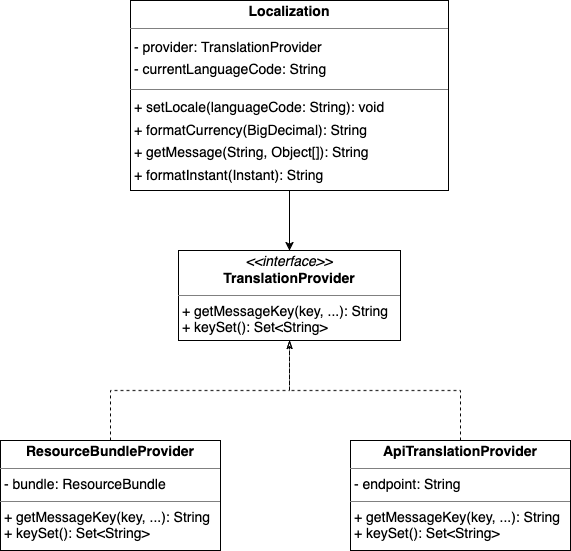
\includegraphics[width=0.65\linewidth]{kapitel3_solid/negative_ocp_neu.drawio.png}
\end{figure}


\subsection{Analyse [LSP/ISP/DIP] (2P)}
\task{jeweils eine Klasse als positives und negatives Beispiel für entweder LSP oder ISP oder DIP;  jeweils UML und Begründung, warum hier das Prinzip erfüllt/nicht erfüllt wird; beim Negativ-Beispiel UML einer möglichen Lösung hinzufügen}
\task{Anm.: es darf nur ein Prinzip ausgewählt werden; es darf NICHT z.B. ein positives Beispiel für LSP und ein negatives Beispiel für ISP genommen werden}
\\
\textbf{Gewähltes Prinzip: ISP}

\subsubsection*{Positiv-Beispiel}
Die Schnittstelle \texttt{BankAccountService} definiert ausschließlich Methoden rund um Bankkonten und hat somit eine sehr saubere Trennung: Die Schnittstelle ist spezifisch und auf eine einzige Domäne fokussiert.
\lstinputlisting[language=Java,style=codeStyle]{kapitel3_solid/ISP_BankAccountService.java}
\textbf{Begründung}
\begin{itemize}
    \item Interface ist spezialisiert und damit gut für Testbarkeit und Wartung
    \item Folgeprinzip: niedrige Kopplung, hohe Kohäsion
\end{itemize}
\textbf{UML}
\begin{figure}[htbp]
    \centering
    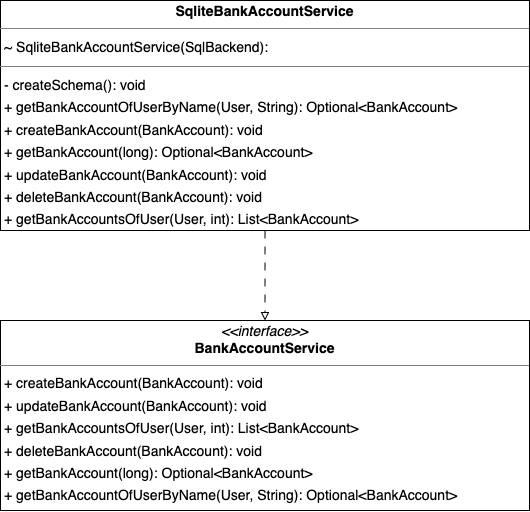
\includegraphics[width=0.65\linewidth]{kapitel3_solid/ISP_pos_bankaccount.drawio.png}
\end{figure}

\subsubsection*{Negativ-Beispiel}
Das Command-Interface wird von allen Befehlen im Terminal verwendet und sieht so aus:
\lstinputlisting[language=Java,style=codeStyle]{kapitel3_solid/ISP_Command.java}
Das wirkt erstmal schlank, aber: In der Praxis gibt es viele Commands, die keine Argumente brauchen, oder deren Verwendung durch das Interface erzwungen wird, obwohl sie sie gar nicht nutzen.
\textbf{Begründung}
\begin{itemize}
    \item Ein Interface sollte nur das vorschreiben, was für den jeweiligen Fall zwingend nötig ist.
    \item \texttt{Command} ist zu allgemein – spezialisierte Commands (z.B. Info-Commands vs. System-Commands) sollten getrennte Interfaces bekommen.
    \item Verstöße gegen ISP führen oft zu optionalen, leeren oder irrelevanten Implementierungen → das ist ein Code-Smell.
\end{itemize}
\textbf{UML - Ist-Zustand}\newline
\begin{figure}[htbp]
    \centering
    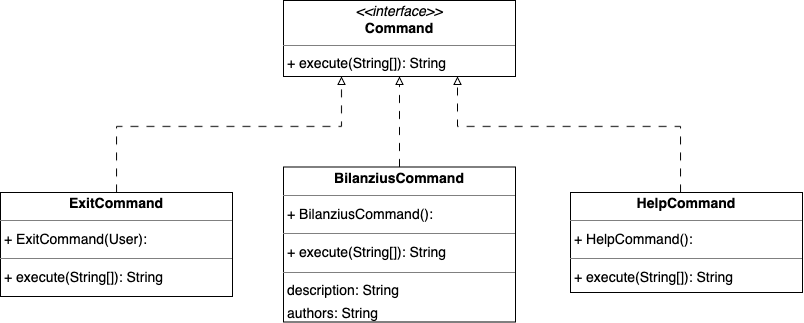
\includegraphics[width=\linewidth]{kapitel3_solid/ISP_neg_Command2.drawio.png}
\end{figure}
\newline
\textbf{Verbesserungsvorschlag}\newline
Trennen von \texttt{Command} in spezifischere Interfaces, z.B.:
\lstinputlisting[language=Java,style=codeStyle]{kapitel3_solid/ISP_Commands.java}
Dann können z.B. \texttt{HelpCommand} und \texttt{ExitCommand} \texttt{SimpleCommand} implementieren, während z.B. ein \textbf{CreateCategoryCommand} ein ArgumentCommand implementiert.\newline\newline
\textbf{UML Verbesserung}
\begin{figure}[htbp]
    \centering
    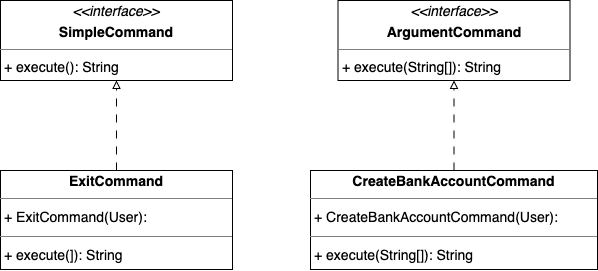
\includegraphics[width=\linewidth]{kapitel3_solid/ISP_neg_betterCommand2.drawio.png}
\end{figure}
\section{SOLID (8P)}

\subsection{Analyse SRP (3P)}
\task{jeweils eine Klasse als positives und negatives Beispiel für SRP; jeweils UML und Beschreibung der Aufgabe bzw. der Aufgaben und möglicher Lösungsweg des Negativ-Beispiels (inkl. UML)}

\subsubsection*{Positiv-Beispiel}
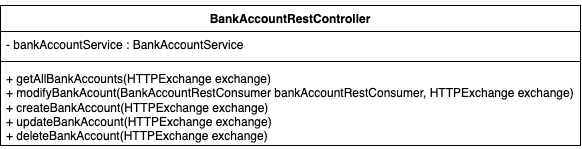
\includegraphics[width=\linewidth]{kapitel3_solid/BankAccountRestController.png}
Der BankAccountRestController ist eine Klasse, welche die CRUD-Endpunkte für die Bankkonten anbietet.

\subsubsection*{Negativ-Beispiel}
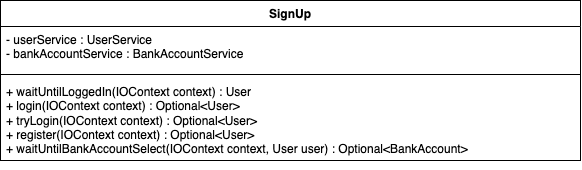
\includegraphics[width=\linewidth]{kapitel3_solid/SignUp.png}
Die SingUp-Klasse ist für das Anmelden und Registrieren eines Benutzers vor dem Programm dar. Dadurch das die Methoden waitUntilLoggedIn() sowie waitUntilBankAccountIsSelect() eher weniger mit dem Anmelden zu tun haben, müsste man diese in eine neue Klasse wie zum Beispiel WaitUntil extrahieren.



\subsection{Analyse OCP (3P)}
\task{jeweils eine Klasse als positives und negatives Beispiel für OCP;  jeweils UML und Analyse mit Begründung, warum das OCP erfüllt/nicht erfüllt wurde – falls erfüllt: warum hier sinnvoll/welches Problem gab es? Falls nicht erfüllt: wie könnte man es lösen (inkl. UML)?}

\subsubsection*{Positiv-Beispiel}
Die Klasse \texttt{HTMLTag} wurde im Projekt als Interface definiert, das eine einheitliche Methode \texttt{build()} bereitstellt. Alle HTML-Komponenten (wie \texttt{HTMLTableRow}, \texttt{HTMLDataCell} oder \texttt{HTMLHeaderCell}) implementieren dieses Interface. Dadurch können neue HTML-Elemente flexibel ergänzt werden, ohne die bestehende Logik anzupassen.
\newline
Beispielsweise kann der \texttt{FinanceReportBuilder} über eine Liste von HTMLTag-Elementen iterieren und sie per \texttt{build()} zu HTML umwandeln. Dies ist dabei unabhängig von der konkreten Implementierung.
\newline
Dieses Design erfüllt das Open/Closed Principle, da die Funktionalität durch neue Klassen erweitert, aber das bestehende Interface und die Verarbeitung nicht verändert werden müssen.
\newline
\textbf{Warum hier sinnvoll?} Das HTML-Reporting soll flexibel auf neue Anforderungen reagieren können (z.B. neue Zeilentypen oder Zellenformate). Mit dem Interface-Ansatz kann dies erfolgen, ohne dass zentrale Komponenten wie der \texttt{ReportBuilder} angepasst werden müssen.
\newline\newline
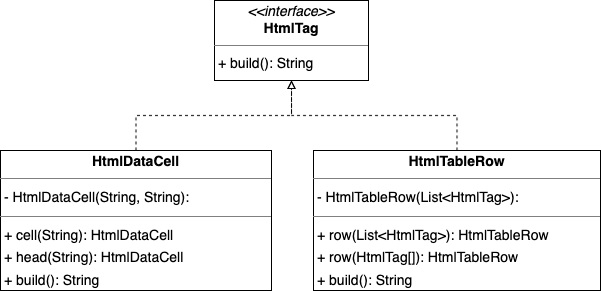
\includegraphics[width=\linewidth]{kapitel3_solid/positive_ocp.png}

\subsubsection*{Negativ Beispiel}
Die Klasse \texttt{Localization} ist für die Übersetzung von Texten in verschiedene Sprachen zuständig. Sie verwendet intern \texttt{ResourceBundle}, um Übersetzungen aus \texttt{.properties}-Dateien basierend auf einem Sprachcode zu laden (\texttt{messages\_en.properties}, \texttt{messages\_de.properties})
\newline\newline
\textbf{Warum wird das OCP hier verletzt?}\newline
Die Klasse ist nicht offen für Erweiterungen, sondern muss bei jeder neuen Anforderung direkt geändert werden. Dadurch verstößt sie gegen das Open/Closed Principle:
\begin{itemize}
    \item Neue Sprachen (z.B. „fr“) müssen im Code zur Liste \texttt{supportedLanguages} hinzugefügt werden.
    \item Neue Übersetzungsquellen (z.B. JSON-Dateien, Datenbank, REST-API) erfordern Änderungen an der Methode \texttt{setLocale(...)}, da dort \texttt{ResourceBundle} fest eingebunden ist.
    \item Eine dynamische Erweiterung oder das Nachladen von Übersetzungen zur Laufzeit ist nicht möglich, ohne die bestehende Klasse zu verändern.
\end{itemize}
\newline
\textbf{Lösungsansatz:}\newline
Um das Open/Closed Principle einzuhalten, sollte die eigentliche Übersetzungslogik in ein Interface ausgelagert werden, z.B. \texttt{TranslationProvider}. Damit könnten unterschiedliche Implementierungen genutzt werden, ohne \texttt{Localization} ändern zu müssen:
\newline
\lstinputlisting[language=Java,style=codeStyle]{kapitel3_solid/translationProvider.java}
Die Localization-Klasse müsste dann nur noch ein solches Interface nutzen – und wäre offen für Erweiterung, aber geschlossen für Modifikation. Beispielhafte Implementierungen könnten dann die folgenden sein: \newline
\begin{itemize}
    \item ResourceBundleTranslationProvider
    \item JsonTranslationProvider
    \item ApiTranslationProvider
\end{itemize}
\subsubsection*{UML-Vergleich}
\textbf{Ist-Zustand:}
\begin{figure}[htbp]
    \centering
    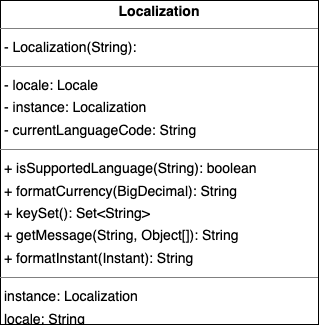
\includegraphics[width=0.5\linewidth]{kapitel3_solid/negative_ocp_ist.drawio.png}
\end{figure}
\newline
\textbf{Nachher:}
\begin{figure}[htbp]
    \centering
    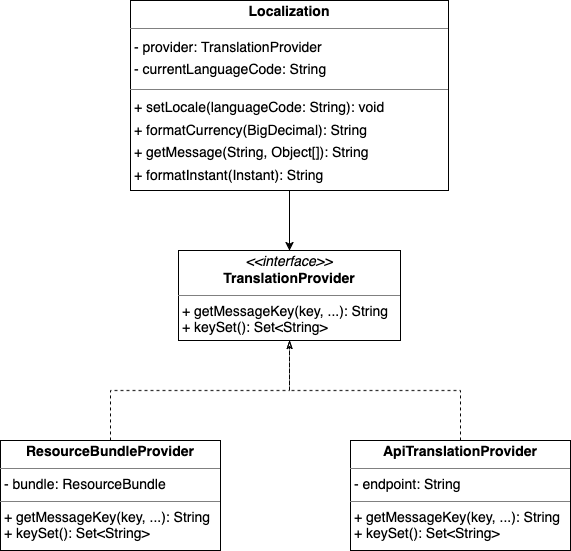
\includegraphics[width=0.65\linewidth]{kapitel3_solid/negative_ocp_neu.drawio.png}
\end{figure}


\subsection{Analyse [LSP/ISP/DIP] (2P)}
\task{jeweils eine Klasse als positives und negatives Beispiel für entweder LSP oder ISP oder DIP;  jeweils UML und Begründung, warum hier das Prinzip erfüllt/nicht erfüllt wird; beim Negativ-Beispiel UML einer möglichen Lösung hinzufügen}
\task{Anm.: es darf nur ein Prinzip ausgewählt werden; es darf NICHT z.B. ein positives Beispiel für LSP und ein negatives Beispiel für ISP genommen werden}
\\
\textbf{Gewähltes Prinzip: ISP}

\subsubsection*{Positiv-Beispiel}
Die Schnittstelle \texttt{BankAccountService} definiert ausschließlich Methoden rund um Bankkonten und hat somit eine sehr saubere Trennung: Die Schnittstelle ist spezifisch und auf eine einzige Domäne fokussiert.
\lstinputlisting[language=Java,style=codeStyle]{kapitel3_solid/ISP_BankAccountService.java}
\textbf{Begründung}
\begin{itemize}
    \item Interface ist spezialisiert und damit gut für Testbarkeit und Wartung
    \item Folgeprinzip: niedrige Kopplung, hohe Kohäsion
\end{itemize}
\textbf{UML}
\begin{figure}[htbp]
    \centering
    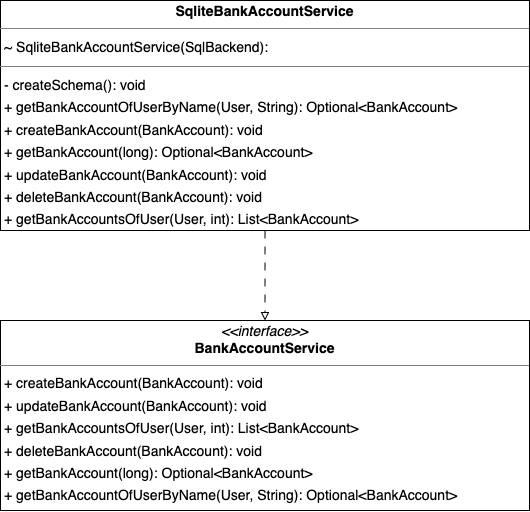
\includegraphics[width=0.65\linewidth]{kapitel3_solid/ISP_pos_bankaccount.drawio.png}
\end{figure}

\subsubsection*{Negativ-Beispiel}
Das Command-Interface wird von allen Befehlen im Terminal verwendet und sieht so aus:
\lstinputlisting[language=Java,style=codeStyle]{kapitel3_solid/ISP_Command.java}
Das wirkt erstmal schlank, aber: In der Praxis gibt es viele Commands, die keine Argumente brauchen, oder deren Verwendung durch das Interface erzwungen wird, obwohl sie sie gar nicht nutzen.
\textbf{Begründung}
\begin{itemize}
    \item Ein Interface sollte nur das vorschreiben, was für den jeweiligen Fall zwingend nötig ist.
    \item \texttt{Command} ist zu allgemein – spezialisierte Commands (z.B. Info-Commands vs. System-Commands) sollten getrennte Interfaces bekommen.
    \item Verstöße gegen ISP führen oft zu optionalen, leeren oder irrelevanten Implementierungen → das ist ein Code-Smell.
\end{itemize}
\textbf{UML - Ist-Zustand}\newline
\begin{figure}[htbp]
    \centering
    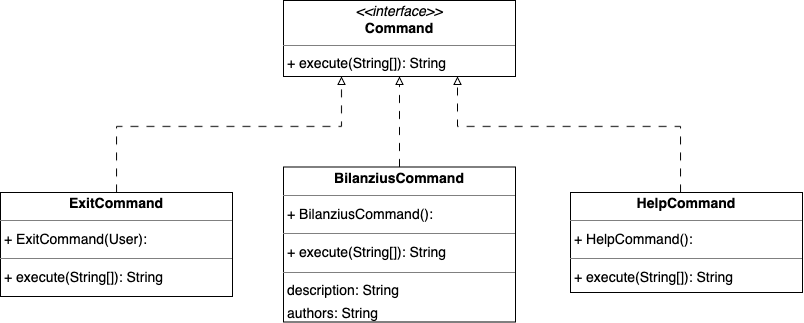
\includegraphics[width=\linewidth]{kapitel3_solid/ISP_neg_Command2.drawio.png}
\end{figure}
\newline
\textbf{Verbesserungsvorschlag}\newline
Trennen von \texttt{Command} in spezifischere Interfaces, z.B.:
\lstinputlisting[language=Java,style=codeStyle]{kapitel3_solid/ISP_Commands.java}
Dann können z.B. \texttt{HelpCommand} und \texttt{ExitCommand} \texttt{SimpleCommand} implementieren, während z.B. ein \textbf{CreateCategoryCommand} ein ArgumentCommand implementiert.\newline\newline
\textbf{UML Verbesserung}
\begin{figure}[htbp]
    \centering
    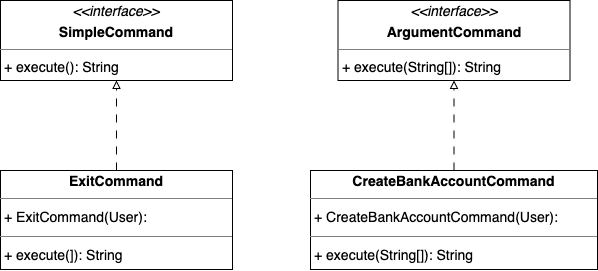
\includegraphics[width=\linewidth]{kapitel3_solid/ISP_neg_betterCommand2.drawio.png}
\end{figure}
\section{SOLID (8P)}

\subsection{Analyse SRP (3P)}
\task{jeweils eine Klasse als positives und negatives Beispiel für SRP; jeweils UML und Beschreibung der Aufgabe bzw. der Aufgaben und möglicher Lösungsweg des Negativ-Beispiels (inkl. UML)}

\subsubsection*{Positiv-Beispiel}
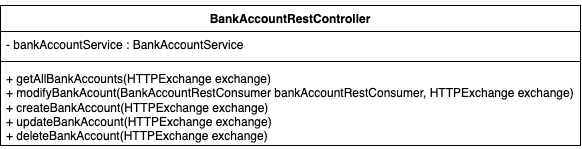
\includegraphics[width=\linewidth]{kapitel3_solid/BankAccountRestController.png}
Der BankAccountRestController ist eine Klasse, welche die CRUD-Endpunkte für die Bankkonten anbietet.

\subsubsection*{Negativ-Beispiel}
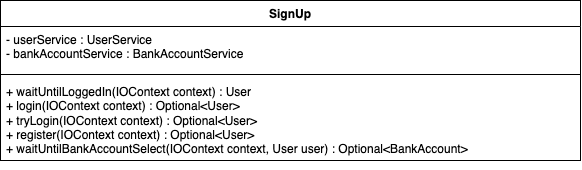
\includegraphics[width=\linewidth]{kapitel3_solid/SignUp.png}
Die SingUp-Klasse ist für das Anmelden und Registrieren eines Benutzers vor dem Programm dar. Dadurch das die Methoden waitUntilLoggedIn() sowie waitUntilBankAccountIsSelect() eher weniger mit dem Anmelden zu tun haben, müsste man diese in eine neue Klasse wie zum Beispiel WaitUntil extrahieren.



\subsection{Analyse OCP (3P)}
\task{jeweils eine Klasse als positives und negatives Beispiel für OCP;  jeweils UML und Analyse mit Begründung, warum das OCP erfüllt/nicht erfüllt wurde – falls erfüllt: warum hier sinnvoll/welches Problem gab es? Falls nicht erfüllt: wie könnte man es lösen (inkl. UML)?}

\subsubsection*{Positiv-Beispiel}
Die Klasse \texttt{HTMLTag} wurde im Projekt als Interface definiert, das eine einheitliche Methode \texttt{build()} bereitstellt. Alle HTML-Komponenten (wie \texttt{HTMLTableRow}, \texttt{HTMLDataCell} oder \texttt{HTMLHeaderCell}) implementieren dieses Interface. Dadurch können neue HTML-Elemente flexibel ergänzt werden, ohne die bestehende Logik anzupassen.
\newline
Beispielsweise kann der \texttt{FinanceReportBuilder} über eine Liste von HTMLTag-Elementen iterieren und sie per \texttt{build()} zu HTML umwandeln. Dies ist dabei unabhängig von der konkreten Implementierung.
\newline
Dieses Design erfüllt das Open/Closed Principle, da die Funktionalität durch neue Klassen erweitert, aber das bestehende Interface und die Verarbeitung nicht verändert werden müssen.
\newline
\textbf{Warum hier sinnvoll?} Das HTML-Reporting soll flexibel auf neue Anforderungen reagieren können (z.B. neue Zeilentypen oder Zellenformate). Mit dem Interface-Ansatz kann dies erfolgen, ohne dass zentrale Komponenten wie der \texttt{ReportBuilder} angepasst werden müssen.
\newline\newline
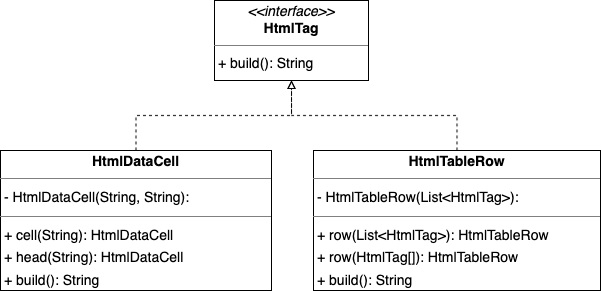
\includegraphics[width=\linewidth]{kapitel3_solid/positive_ocp.png}

\subsubsection*{Negativ Beispiel}
Die Klasse \texttt{Localization} ist für die Übersetzung von Texten in verschiedene Sprachen zuständig. Sie verwendet intern \texttt{ResourceBundle}, um Übersetzungen aus \texttt{.properties}-Dateien basierend auf einem Sprachcode zu laden (\texttt{messages\_en.properties}, \texttt{messages\_de.properties})
\newline\newline
\textbf{Warum wird das OCP hier verletzt?}\newline
Die Klasse ist nicht offen für Erweiterungen, sondern muss bei jeder neuen Anforderung direkt geändert werden. Dadurch verstößt sie gegen das Open/Closed Principle:
\begin{itemize}
    \item Neue Sprachen (z.B. „fr“) müssen im Code zur Liste \texttt{supportedLanguages} hinzugefügt werden.
    \item Neue Übersetzungsquellen (z.B. JSON-Dateien, Datenbank, REST-API) erfordern Änderungen an der Methode \texttt{setLocale(...)}, da dort \texttt{ResourceBundle} fest eingebunden ist.
    \item Eine dynamische Erweiterung oder das Nachladen von Übersetzungen zur Laufzeit ist nicht möglich, ohne die bestehende Klasse zu verändern.
\end{itemize}
\newline
\textbf{Lösungsansatz:}\newline
Um das Open/Closed Principle einzuhalten, sollte die eigentliche Übersetzungslogik in ein Interface ausgelagert werden, z.B. \texttt{TranslationProvider}. Damit könnten unterschiedliche Implementierungen genutzt werden, ohne \texttt{Localization} ändern zu müssen:
\newline
\lstinputlisting[language=Java,style=codeStyle]{kapitel3_solid/translationProvider.java}
Die Localization-Klasse müsste dann nur noch ein solches Interface nutzen – und wäre offen für Erweiterung, aber geschlossen für Modifikation. Beispielhafte Implementierungen könnten dann die folgenden sein: \newline
\begin{itemize}
    \item ResourceBundleTranslationProvider
    \item JsonTranslationProvider
    \item ApiTranslationProvider
\end{itemize}
\subsubsection*{UML-Vergleich}
\textbf{Ist-Zustand:}
\begin{figure}[htbp]
    \centering
    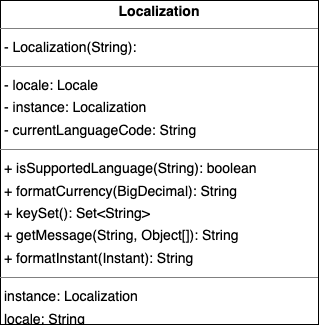
\includegraphics[width=0.5\linewidth]{kapitel3_solid/negative_ocp_ist.drawio.png}
\end{figure}
\newline
\textbf{Nachher:}
\begin{figure}[htbp]
    \centering
    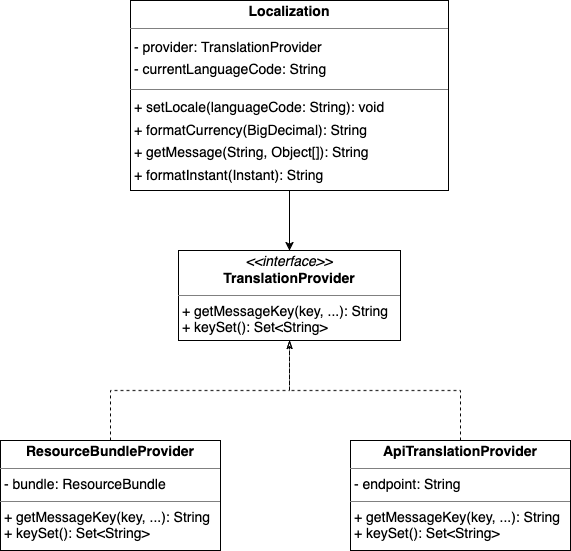
\includegraphics[width=0.65\linewidth]{kapitel3_solid/negative_ocp_neu.drawio.png}
\end{figure}


\subsection{Analyse [LSP/ISP/DIP] (2P)}
\task{jeweils eine Klasse als positives und negatives Beispiel für entweder LSP oder ISP oder DIP;  jeweils UML und Begründung, warum hier das Prinzip erfüllt/nicht erfüllt wird; beim Negativ-Beispiel UML einer möglichen Lösung hinzufügen}
\task{Anm.: es darf nur ein Prinzip ausgewählt werden; es darf NICHT z.B. ein positives Beispiel für LSP und ein negatives Beispiel für ISP genommen werden}
\\
\textbf{Gewähltes Prinzip: ISP}

\subsubsection*{Positiv-Beispiel}
Die Schnittstelle \texttt{BankAccountService} definiert ausschließlich Methoden rund um Bankkonten und hat somit eine sehr saubere Trennung: Die Schnittstelle ist spezifisch und auf eine einzige Domäne fokussiert.
\lstinputlisting[language=Java,style=codeStyle]{kapitel3_solid/ISP_BankAccountService.java}
\textbf{Begründung}
\begin{itemize}
    \item Interface ist spezialisiert und damit gut für Testbarkeit und Wartung
    \item Folgeprinzip: niedrige Kopplung, hohe Kohäsion
\end{itemize}
\textbf{UML}
\begin{figure}[htbp]
    \centering
    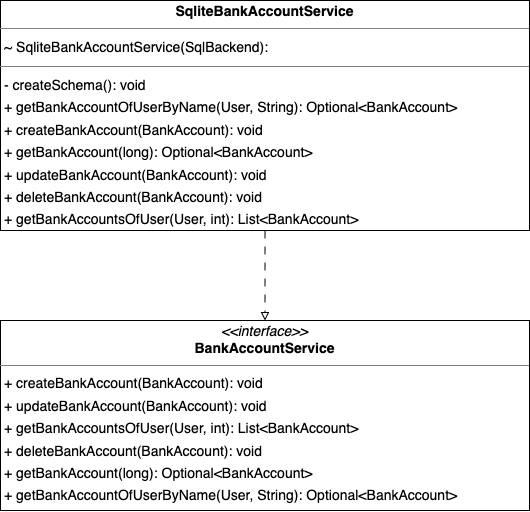
\includegraphics[width=0.65\linewidth]{kapitel3_solid/ISP_pos_bankaccount.drawio.png}
\end{figure}

\subsubsection*{Negativ-Beispiel}
Das Command-Interface wird von allen Befehlen im Terminal verwendet und sieht so aus:
\lstinputlisting[language=Java,style=codeStyle]{kapitel3_solid/ISP_Command.java}
Das wirkt erstmal schlank, aber: In der Praxis gibt es viele Commands, die keine Argumente brauchen, oder deren Verwendung durch das Interface erzwungen wird, obwohl sie sie gar nicht nutzen.
\textbf{Begründung}
\begin{itemize}
    \item Ein Interface sollte nur das vorschreiben, was für den jeweiligen Fall zwingend nötig ist.
    \item \texttt{Command} ist zu allgemein – spezialisierte Commands (z.B. Info-Commands vs. System-Commands) sollten getrennte Interfaces bekommen.
    \item Verstöße gegen ISP führen oft zu optionalen, leeren oder irrelevanten Implementierungen → das ist ein Code-Smell.
\end{itemize}
\textbf{UML - Ist-Zustand}\newline
\begin{figure}[htbp]
    \centering
    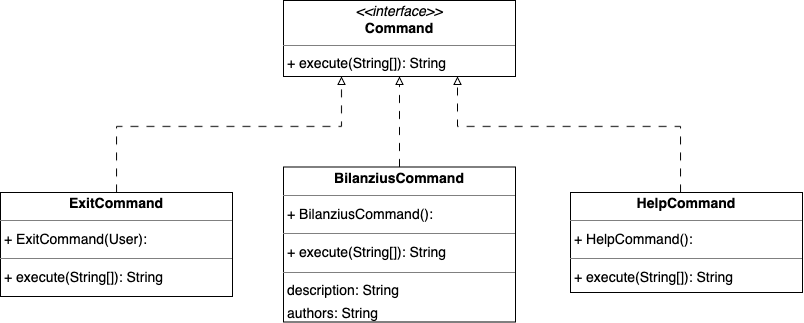
\includegraphics[width=\linewidth]{kapitel3_solid/ISP_neg_Command2.drawio.png}
\end{figure}
\newline
\textbf{Verbesserungsvorschlag}\newline
Trennen von \texttt{Command} in spezifischere Interfaces, z.B.:
\lstinputlisting[language=Java,style=codeStyle]{kapitel3_solid/ISP_Commands.java}
Dann können z.B. \texttt{HelpCommand} und \texttt{ExitCommand} \texttt{SimpleCommand} implementieren, während z.B. ein \textbf{CreateCategoryCommand} ein ArgumentCommand implementiert.\newline\newline
\textbf{UML Verbesserung}
\begin{figure}[htbp]
    \centering
    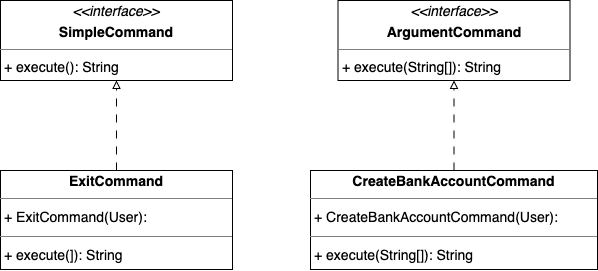
\includegraphics[width=\linewidth]{kapitel3_solid/ISP_neg_betterCommand2.drawio.png}
\end{figure}
\section{SOLID (8P)}

\subsection{Analyse SRP (3P)}
\task{jeweils eine Klasse als positives und negatives Beispiel für SRP; jeweils UML und Beschreibung der Aufgabe bzw. der Aufgaben und möglicher Lösungsweg des Negativ-Beispiels (inkl. UML)}

\subsubsection*{Positiv-Beispiel}
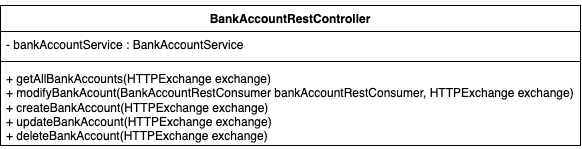
\includegraphics[width=\linewidth]{kapitel3_solid/BankAccountRestController.png}
Der BankAccountRestController ist eine Klasse, welche die CRUD-Endpunkte für die Bankkonten anbietet.

\subsubsection*{Negativ-Beispiel}
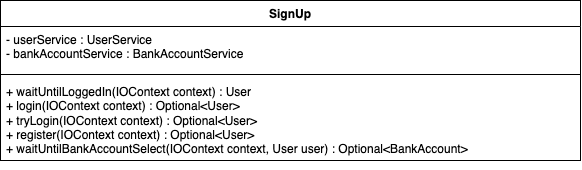
\includegraphics[width=\linewidth]{kapitel3_solid/SignUp.png}
Die SingUp-Klasse ist für das Anmelden und Registrieren eines Benutzers vor dem Programm dar. Dadurch das die Methoden waitUntilLoggedIn() sowie waitUntilBankAccountIsSelect() eher weniger mit dem Anmelden zu tun haben, müsste man diese in eine neue Klasse wie zum Beispiel WaitUntil extrahieren.



\subsection{Analyse OCP (3P)}
\task{jeweils eine Klasse als positives und negatives Beispiel für OCP;  jeweils UML und Analyse mit Begründung, warum das OCP erfüllt/nicht erfüllt wurde – falls erfüllt: warum hier sinnvoll/welches Problem gab es? Falls nicht erfüllt: wie könnte man es lösen (inkl. UML)?}

\subsubsection*{Positiv-Beispiel}
Die Klasse \texttt{HTMLTag} wurde im Projekt als Interface definiert, das eine einheitliche Methode \texttt{build()} bereitstellt. Alle HTML-Komponenten (wie \texttt{HTMLTableRow}, \texttt{HTMLDataCell} oder \texttt{HTMLHeaderCell}) implementieren dieses Interface. Dadurch können neue HTML-Elemente flexibel ergänzt werden, ohne die bestehende Logik anzupassen.
\newline
Beispielsweise kann der \texttt{FinanceReportBuilder} über eine Liste von HTMLTag-Elementen iterieren und sie per \texttt{build()} zu HTML umwandeln. Dies ist dabei unabhängig von der konkreten Implementierung.
\newline
Dieses Design erfüllt das Open/Closed Principle, da die Funktionalität durch neue Klassen erweitert, aber das bestehende Interface und die Verarbeitung nicht verändert werden müssen.
\newline
\textbf{Warum hier sinnvoll?} Das HTML-Reporting soll flexibel auf neue Anforderungen reagieren können (z.B. neue Zeilentypen oder Zellenformate). Mit dem Interface-Ansatz kann dies erfolgen, ohne dass zentrale Komponenten wie der \texttt{ReportBuilder} angepasst werden müssen.
\newline\newline
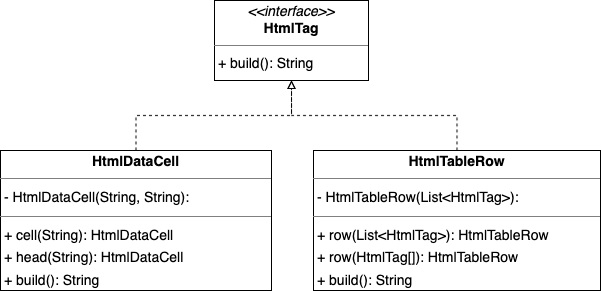
\includegraphics[width=\linewidth]{kapitel3_solid/positive_ocp.png}

\subsubsection*{Negativ Beispiel}
Die Klasse \texttt{Localization} ist für die Übersetzung von Texten in verschiedene Sprachen zuständig. Sie verwendet intern \texttt{ResourceBundle}, um Übersetzungen aus \texttt{.properties}-Dateien basierend auf einem Sprachcode zu laden (\texttt{messages\_en.properties}, \texttt{messages\_de.properties})
\newline\newline
\textbf{Warum wird das OCP hier verletzt?}\newline
Die Klasse ist nicht offen für Erweiterungen, sondern muss bei jeder neuen Anforderung direkt geändert werden. Dadurch verstößt sie gegen das Open/Closed Principle:
\begin{itemize}
    \item Neue Sprachen (z.B. „fr“) müssen im Code zur Liste \texttt{supportedLanguages} hinzugefügt werden.
    \item Neue Übersetzungsquellen (z.B. JSON-Dateien, Datenbank, REST-API) erfordern Änderungen an der Methode \texttt{setLocale(...)}, da dort \texttt{ResourceBundle} fest eingebunden ist.
    \item Eine dynamische Erweiterung oder das Nachladen von Übersetzungen zur Laufzeit ist nicht möglich, ohne die bestehende Klasse zu verändern.
\end{itemize}
\newline
\textbf{Lösungsansatz:}\newline
Um das Open/Closed Principle einzuhalten, sollte die eigentliche Übersetzungslogik in ein Interface ausgelagert werden, z.B. \texttt{TranslationProvider}. Damit könnten unterschiedliche Implementierungen genutzt werden, ohne \texttt{Localization} ändern zu müssen:
\newline
\lstinputlisting[language=Java,style=codeStyle]{kapitel3_solid/translationProvider.java}
Die Localization-Klasse müsste dann nur noch ein solches Interface nutzen – und wäre offen für Erweiterung, aber geschlossen für Modifikation. Beispielhafte Implementierungen könnten dann die folgenden sein: \newline
\begin{itemize}
    \item ResourceBundleTranslationProvider
    \item JsonTranslationProvider
    \item ApiTranslationProvider
\end{itemize}
\subsubsection*{UML-Vergleich}
\textbf{Ist-Zustand:}
\begin{figure}[htbp]
    \centering
    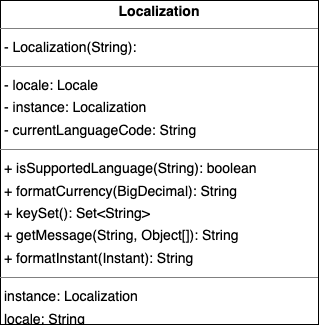
\includegraphics[width=0.5\linewidth]{kapitel3_solid/negative_ocp_ist.drawio.png}
\end{figure}
\newline
\textbf{Nachher:}
\begin{figure}[htbp]
    \centering
    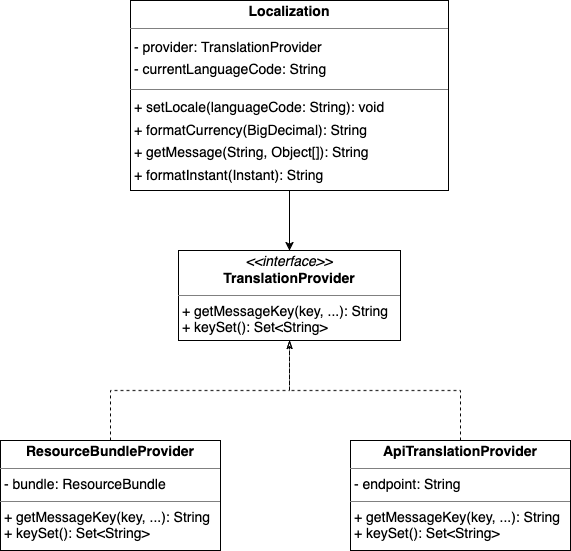
\includegraphics[width=0.65\linewidth]{kapitel3_solid/negative_ocp_neu.drawio.png}
\end{figure}


\subsection{Analyse [LSP/ISP/DIP] (2P)}
\task{jeweils eine Klasse als positives und negatives Beispiel für entweder LSP oder ISP oder DIP;  jeweils UML und Begründung, warum hier das Prinzip erfüllt/nicht erfüllt wird; beim Negativ-Beispiel UML einer möglichen Lösung hinzufügen}
\task{Anm.: es darf nur ein Prinzip ausgewählt werden; es darf NICHT z.B. ein positives Beispiel für LSP und ein negatives Beispiel für ISP genommen werden}
\\
\textbf{Gewähltes Prinzip: ISP}

\subsubsection*{Positiv-Beispiel}
Die Schnittstelle \texttt{BankAccountService} definiert ausschließlich Methoden rund um Bankkonten und hat somit eine sehr saubere Trennung: Die Schnittstelle ist spezifisch und auf eine einzige Domäne fokussiert.
\lstinputlisting[language=Java,style=codeStyle]{kapitel3_solid/ISP_BankAccountService.java}
\textbf{Begründung}
\begin{itemize}
    \item Interface ist spezialisiert und damit gut für Testbarkeit und Wartung
    \item Folgeprinzip: niedrige Kopplung, hohe Kohäsion
\end{itemize}
\textbf{UML}
\begin{figure}[htbp]
    \centering
    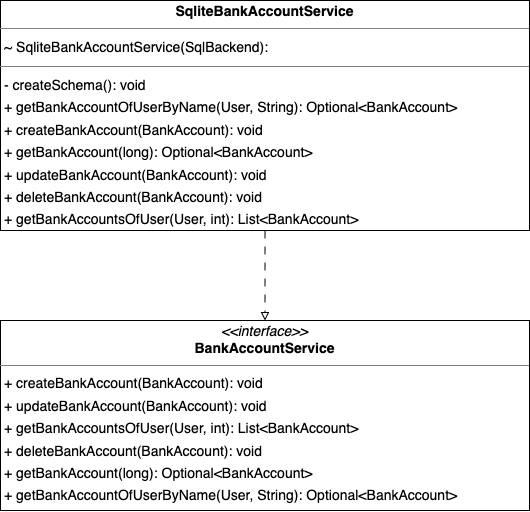
\includegraphics[width=0.65\linewidth]{kapitel3_solid/ISP_pos_bankaccount.drawio.png}
\end{figure}

\subsubsection*{Negativ-Beispiel}
Das Command-Interface wird von allen Befehlen im Terminal verwendet und sieht so aus:
\lstinputlisting[language=Java,style=codeStyle]{kapitel3_solid/ISP_Command.java}
Das wirkt erstmal schlank, aber: In der Praxis gibt es viele Commands, die keine Argumente brauchen, oder deren Verwendung durch das Interface erzwungen wird, obwohl sie sie gar nicht nutzen.
\textbf{Begründung}
\begin{itemize}
    \item Ein Interface sollte nur das vorschreiben, was für den jeweiligen Fall zwingend nötig ist.
    \item \texttt{Command} ist zu allgemein – spezialisierte Commands (z.B. Info-Commands vs. System-Commands) sollten getrennte Interfaces bekommen.
    \item Verstöße gegen ISP führen oft zu optionalen, leeren oder irrelevanten Implementierungen → das ist ein Code-Smell.
\end{itemize}
\textbf{UML - Ist-Zustand}\newline
\begin{figure}[htbp]
    \centering
    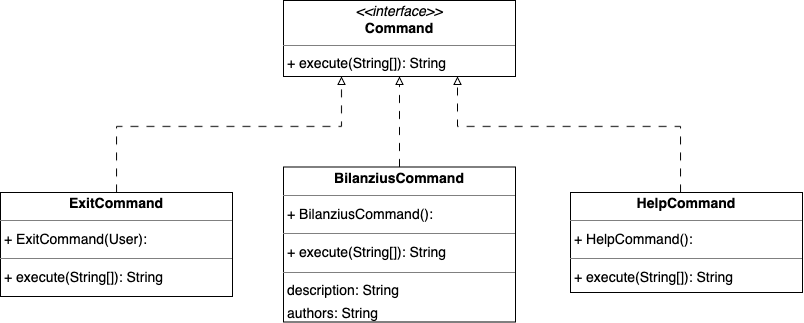
\includegraphics[width=\linewidth]{kapitel3_solid/ISP_neg_Command2.drawio.png}
\end{figure}
\newline
\textbf{Verbesserungsvorschlag}\newline
Trennen von \texttt{Command} in spezifischere Interfaces, z.B.:
\lstinputlisting[language=Java,style=codeStyle]{kapitel3_solid/ISP_Commands.java}
Dann können z.B. \texttt{HelpCommand} und \texttt{ExitCommand} \texttt{SimpleCommand} implementieren, während z.B. ein \textbf{CreateCategoryCommand} ein ArgumentCommand implementiert.\newline\newline
\textbf{UML Verbesserung}
\begin{figure}[htbp]
    \centering
    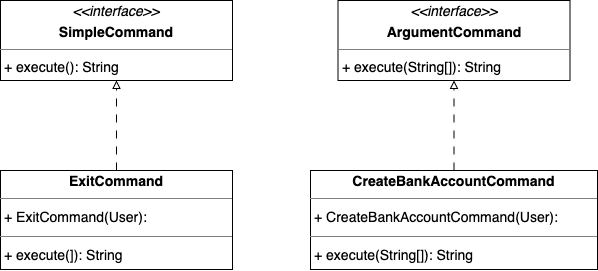
\includegraphics[width=\linewidth]{kapitel3_solid/ISP_neg_betterCommand2.drawio.png}
\end{figure}
\section{SOLID (8P)}

\subsection{Analyse SRP (3P)}
\task{jeweils eine Klasse als positives und negatives Beispiel für SRP; jeweils UML und Beschreibung der Aufgabe bzw. der Aufgaben und möglicher Lösungsweg des Negativ-Beispiels (inkl. UML)}

\subsubsection*{Positiv-Beispiel}
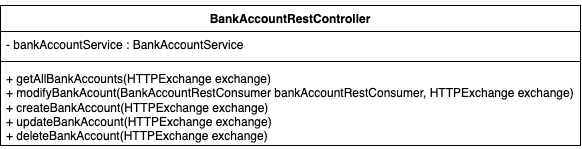
\includegraphics[width=\linewidth]{kapitel3_solid/BankAccountRestController.png}
Der BankAccountRestController ist eine Klasse, welche die CRUD-Endpunkte für die Bankkonten anbietet.

\subsubsection*{Negativ-Beispiel}
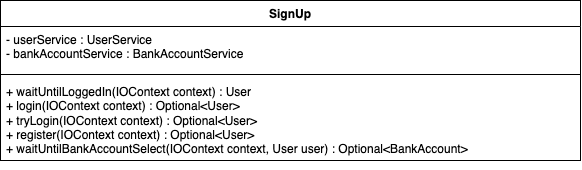
\includegraphics[width=\linewidth]{kapitel3_solid/SignUp.png}
Die SingUp-Klasse ist für das Anmelden und Registrieren eines Benutzers vor dem Programm dar. Dadurch das die Methoden waitUntilLoggedIn() sowie waitUntilBankAccountIsSelect() eher weniger mit dem Anmelden zu tun haben, müsste man diese in eine neue Klasse wie zum Beispiel WaitUntil extrahieren.



\subsection{Analyse OCP (3P)}
\task{jeweils eine Klasse als positives und negatives Beispiel für OCP;  jeweils UML und Analyse mit Begründung, warum das OCP erfüllt/nicht erfüllt wurde – falls erfüllt: warum hier sinnvoll/welches Problem gab es? Falls nicht erfüllt: wie könnte man es lösen (inkl. UML)?}

\subsubsection*{Positiv-Beispiel}
Die Klasse \texttt{HTMLTag} wurde im Projekt als Interface definiert, das eine einheitliche Methode \texttt{build()} bereitstellt. Alle HTML-Komponenten (wie \texttt{HTMLTableRow}, \texttt{HTMLDataCell} oder \texttt{HTMLHeaderCell}) implementieren dieses Interface. Dadurch können neue HTML-Elemente flexibel ergänzt werden, ohne die bestehende Logik anzupassen.
\newline
Beispielsweise kann der \texttt{FinanceReportBuilder} über eine Liste von HTMLTag-Elementen iterieren und sie per \texttt{build()} zu HTML umwandeln. Dies ist dabei unabhängig von der konkreten Implementierung.
\newline
Dieses Design erfüllt das Open/Closed Principle, da die Funktionalität durch neue Klassen erweitert, aber das bestehende Interface und die Verarbeitung nicht verändert werden müssen.
\newline
\textbf{Warum hier sinnvoll?} Das HTML-Reporting soll flexibel auf neue Anforderungen reagieren können (z.B. neue Zeilentypen oder Zellenformate). Mit dem Interface-Ansatz kann dies erfolgen, ohne dass zentrale Komponenten wie der \texttt{ReportBuilder} angepasst werden müssen.
\newline\newline
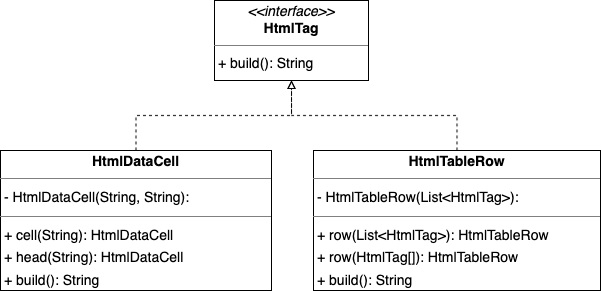
\includegraphics[width=\linewidth]{kapitel3_solid/positive_ocp.png}

\subsubsection*{Negativ Beispiel}
Die Klasse \texttt{Localization} ist für die Übersetzung von Texten in verschiedene Sprachen zuständig. Sie verwendet intern \texttt{ResourceBundle}, um Übersetzungen aus \texttt{.properties}-Dateien basierend auf einem Sprachcode zu laden (\texttt{messages\_en.properties}, \texttt{messages\_de.properties})
\newline\newline
\textbf{Warum wird das OCP hier verletzt?}\newline
Die Klasse ist nicht offen für Erweiterungen, sondern muss bei jeder neuen Anforderung direkt geändert werden. Dadurch verstößt sie gegen das Open/Closed Principle:
\begin{itemize}
    \item Neue Sprachen (z.B. „fr“) müssen im Code zur Liste \texttt{supportedLanguages} hinzugefügt werden.
    \item Neue Übersetzungsquellen (z.B. JSON-Dateien, Datenbank, REST-API) erfordern Änderungen an der Methode \texttt{setLocale(...)}, da dort \texttt{ResourceBundle} fest eingebunden ist.
    \item Eine dynamische Erweiterung oder das Nachladen von Übersetzungen zur Laufzeit ist nicht möglich, ohne die bestehende Klasse zu verändern.
\end{itemize}
\newline
\textbf{Lösungsansatz:}\newline
Um das Open/Closed Principle einzuhalten, sollte die eigentliche Übersetzungslogik in ein Interface ausgelagert werden, z.B. \texttt{TranslationProvider}. Damit könnten unterschiedliche Implementierungen genutzt werden, ohne \texttt{Localization} ändern zu müssen:
\newline
\lstinputlisting[language=Java,style=codeStyle]{kapitel3_solid/translationProvider.java}
Die Localization-Klasse müsste dann nur noch ein solches Interface nutzen – und wäre offen für Erweiterung, aber geschlossen für Modifikation. Beispielhafte Implementierungen könnten dann die folgenden sein: \newline
\begin{itemize}
    \item ResourceBundleTranslationProvider
    \item JsonTranslationProvider
    \item ApiTranslationProvider
\end{itemize}
\subsubsection*{UML-Vergleich}
\textbf{Ist-Zustand:}
\begin{figure}[htbp]
    \centering
    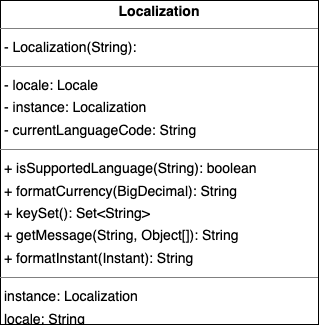
\includegraphics[width=0.5\linewidth]{kapitel3_solid/negative_ocp_ist.drawio.png}
\end{figure}
\newline
\textbf{Nachher:}
\begin{figure}[htbp]
    \centering
    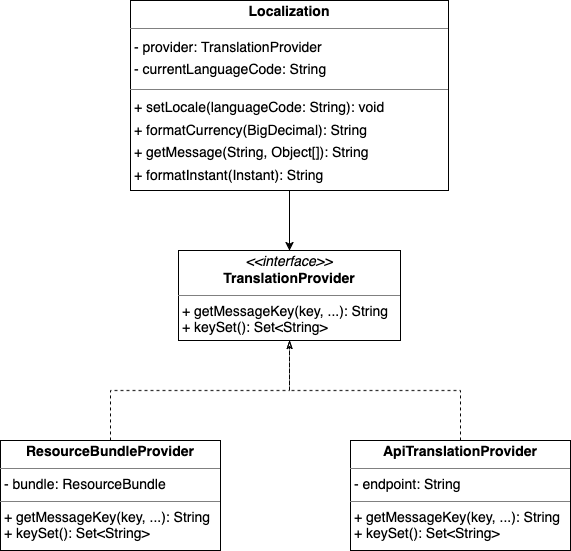
\includegraphics[width=0.65\linewidth]{kapitel3_solid/negative_ocp_neu.drawio.png}
\end{figure}


\subsection{Analyse [LSP/ISP/DIP] (2P)}
\task{jeweils eine Klasse als positives und negatives Beispiel für entweder LSP oder ISP oder DIP;  jeweils UML und Begründung, warum hier das Prinzip erfüllt/nicht erfüllt wird; beim Negativ-Beispiel UML einer möglichen Lösung hinzufügen}
\task{Anm.: es darf nur ein Prinzip ausgewählt werden; es darf NICHT z.B. ein positives Beispiel für LSP und ein negatives Beispiel für ISP genommen werden}
\\
\textbf{Gewähltes Prinzip: ISP}

\subsubsection*{Positiv-Beispiel}
Die Schnittstelle \texttt{BankAccountService} definiert ausschließlich Methoden rund um Bankkonten und hat somit eine sehr saubere Trennung: Die Schnittstelle ist spezifisch und auf eine einzige Domäne fokussiert.
\lstinputlisting[language=Java,style=codeStyle]{kapitel3_solid/ISP_BankAccountService.java}
\textbf{Begründung}
\begin{itemize}
    \item Interface ist spezialisiert und damit gut für Testbarkeit und Wartung
    \item Folgeprinzip: niedrige Kopplung, hohe Kohäsion
\end{itemize}
\textbf{UML}
\begin{figure}[htbp]
    \centering
    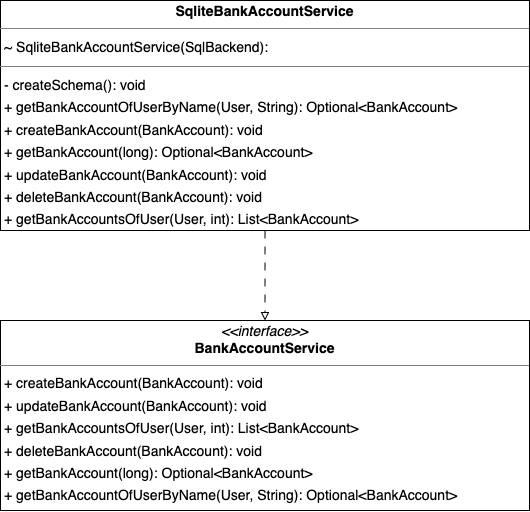
\includegraphics[width=0.65\linewidth]{kapitel3_solid/ISP_pos_bankaccount.drawio.png}
\end{figure}

\subsubsection*{Negativ-Beispiel}
Das Command-Interface wird von allen Befehlen im Terminal verwendet und sieht so aus:
\lstinputlisting[language=Java,style=codeStyle]{kapitel3_solid/ISP_Command.java}
Das wirkt erstmal schlank, aber: In der Praxis gibt es viele Commands, die keine Argumente brauchen, oder deren Verwendung durch das Interface erzwungen wird, obwohl sie sie gar nicht nutzen.
\textbf{Begründung}
\begin{itemize}
    \item Ein Interface sollte nur das vorschreiben, was für den jeweiligen Fall zwingend nötig ist.
    \item \texttt{Command} ist zu allgemein – spezialisierte Commands (z.B. Info-Commands vs. System-Commands) sollten getrennte Interfaces bekommen.
    \item Verstöße gegen ISP führen oft zu optionalen, leeren oder irrelevanten Implementierungen → das ist ein Code-Smell.
\end{itemize}
\textbf{UML - Ist-Zustand}\newline
\begin{figure}[htbp]
    \centering
    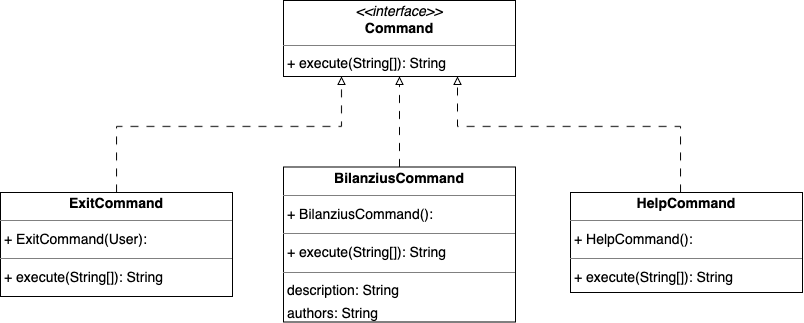
\includegraphics[width=\linewidth]{kapitel3_solid/ISP_neg_Command2.drawio.png}
\end{figure}
\newline
\textbf{Verbesserungsvorschlag}\newline
Trennen von \texttt{Command} in spezifischere Interfaces, z.B.:
\lstinputlisting[language=Java,style=codeStyle]{kapitel3_solid/ISP_Commands.java}
Dann können z.B. \texttt{HelpCommand} und \texttt{ExitCommand} \texttt{SimpleCommand} implementieren, während z.B. ein \textbf{CreateCategoryCommand} ein ArgumentCommand implementiert.\newline\newline
\textbf{UML Verbesserung}
\begin{figure}[htbp]
    \centering
    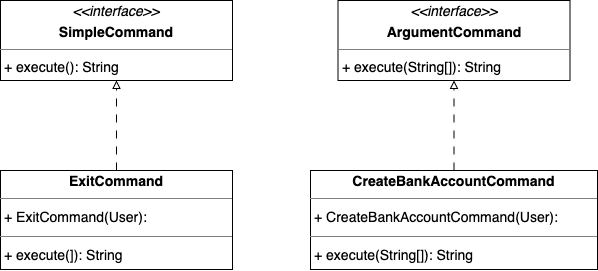
\includegraphics[width=\linewidth]{kapitel3_solid/ISP_neg_betterCommand2.drawio.png}
\end{figure}
\section{SOLID (8P)}

\subsection{Analyse SRP (3P)}
\task{jeweils eine Klasse als positives und negatives Beispiel für SRP; jeweils UML und Beschreibung der Aufgabe bzw. der Aufgaben und möglicher Lösungsweg des Negativ-Beispiels (inkl. UML)}

\subsubsection*{Positiv-Beispiel}
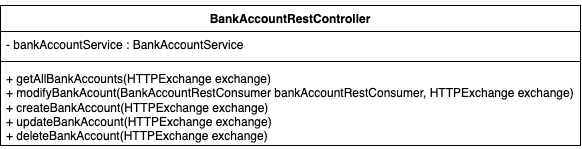
\includegraphics[width=\linewidth]{kapitel3_solid/BankAccountRestController.png}
Der BankAccountRestController ist eine Klasse, welche die CRUD-Endpunkte für die Bankkonten anbietet.

\subsubsection*{Negativ-Beispiel}
\includegraphics[width=\linewidth]{kapitel3_solid/SignUp.png}
Die SingUp-Klasse ist für das Anmelden und Registrieren eines Benutzers vor dem Programm dar. Dadurch das die Methoden waitUntilLoggedIn() sowie waitUntilBankAccountIsSelect() eher weniger mit dem Anmelden zu tun haben, müsste man diese in eine neue Klasse wie zum Beispiel WaitUntil extrahieren.



\subsection{Analyse OCP (3P)}
\task{jeweils eine Klasse als positives und negatives Beispiel für OCP;  jeweils UML und Analyse mit Begründung, warum das OCP erfüllt/nicht erfüllt wurde – falls erfüllt: warum hier sinnvoll/welches Problem gab es? Falls nicht erfüllt: wie könnte man es lösen (inkl. UML)?}

\subsubsection*{Positiv-Beispiel}
Die Klasse \texttt{HTMLTag} wurde im Projekt als Interface definiert, das eine einheitliche Methode \texttt{build()} bereitstellt. Alle HTML-Komponenten (wie \texttt{HTMLTableRow}, \texttt{HTMLDataCell} oder \texttt{HTMLHeaderCell}) implementieren dieses Interface. Dadurch können neue HTML-Elemente flexibel ergänzt werden, ohne die bestehende Logik anzupassen.
\newline
Beispielsweise kann der \texttt{FinanceReportBuilder} über eine Liste von HTMLTag-Elementen iterieren und sie per \texttt{build()} zu HTML umwandeln. Dies ist dabei unabhängig von der konkreten Implementierung.
\newline
Dieses Design erfüllt das Open/Closed Principle, da die Funktionalität durch neue Klassen erweitert, aber das bestehende Interface und die Verarbeitung nicht verändert werden müssen.
\newline
\textbf{Warum hier sinnvoll?} Das HTML-Reporting soll flexibel auf neue Anforderungen reagieren können (z.B. neue Zeilentypen oder Zellenformate). Mit dem Interface-Ansatz kann dies erfolgen, ohne dass zentrale Komponenten wie der \texttt{ReportBuilder} angepasst werden müssen.
\newline\newline
\includegraphics[width=\linewidth]{kapitel3_solid/positive_ocp.png}

\subsubsection*{Negativ Beispiel}
Die Klasse \texttt{Localization} ist für die Übersetzung von Texten in verschiedene Sprachen zuständig. Sie verwendet intern \texttt{ResourceBundle}, um Übersetzungen aus \texttt{.properties}-Dateien basierend auf einem Sprachcode zu laden (\texttt{messages\_en.properties}, \texttt{messages\_de.properties})
\newline\newline
\textbf{Warum wird das OCP hier verletzt?}\newline
Die Klasse ist nicht offen für Erweiterungen, sondern muss bei jeder neuen Anforderung direkt geändert werden. Dadurch verstößt sie gegen das Open/Closed Principle:
\begin{itemize}
    \item Neue Sprachen (z.B. „fr“) müssen im Code zur Liste \texttt{supportedLanguages} hinzugefügt werden.
    \item Neue Übersetzungsquellen (z.B. JSON-Dateien, Datenbank, REST-API) erfordern Änderungen an der Methode \texttt{setLocale(...)}, da dort \texttt{ResourceBundle} fest eingebunden ist.
    \item Eine dynamische Erweiterung oder das Nachladen von Übersetzungen zur Laufzeit ist nicht möglich, ohne die bestehende Klasse zu verändern.
\end{itemize}
\newline
\textbf{Lösungsansatz:}\newline
Um das Open/Closed Principle einzuhalten, sollte die eigentliche Übersetzungslogik in ein Interface ausgelagert werden, z.B. \texttt{TranslationProvider}. Damit könnten unterschiedliche Implementierungen genutzt werden, ohne \texttt{Localization} ändern zu müssen:
\newline
\lstinputlisting[language=Java,style=codeStyle]{kapitel3_solid/translationProvider.java}
Die Localization-Klasse müsste dann nur noch ein solches Interface nutzen – und wäre offen für Erweiterung, aber geschlossen für Modifikation. Beispielhafte Implementierungen könnten dann die folgenden sein: \newline
\begin{itemize}
    \item ResourceBundleTranslationProvider
    \item JsonTranslationProvider
    \item ApiTranslationProvider
\end{itemize}
\subsubsection*{UML-Vergleich}
\textbf{Ist-Zustand:}
\begin{figure}[htbp]
    \centering
    \includegraphics[width=0.5\linewidth]{kapitel3_solid/negative_ocp_ist.drawio.png}
\end{figure}
\newline
\textbf{Nachher:}
\begin{figure}[htbp]
    \centering
    \includegraphics[width=0.65\linewidth]{kapitel3_solid/negative_ocp_neu.drawio.png}
\end{figure}


\subsection{Analyse [LSP/ISP/DIP] (2P)}
\task{jeweils eine Klasse als positives und negatives Beispiel für entweder LSP oder ISP oder DIP;  jeweils UML und Begründung, warum hier das Prinzip erfüllt/nicht erfüllt wird; beim Negativ-Beispiel UML einer möglichen Lösung hinzufügen}
\task{Anm.: es darf nur ein Prinzip ausgewählt werden; es darf NICHT z.B. ein positives Beispiel für LSP und ein negatives Beispiel für ISP genommen werden}
\\
\textbf{Gewähltes Prinzip: ISP}

\subsubsection*{Positiv-Beispiel}
Die Schnittstelle \texttt{BankAccountService} definiert ausschließlich Methoden rund um Bankkonten und hat somit eine sehr saubere Trennung: Die Schnittstelle ist spezifisch und auf eine einzige Domäne fokussiert.
\lstinputlisting[language=Java,style=codeStyle]{kapitel3_solid/ISP_BankAccountService.java}
\textbf{Begründung}
\begin{itemize}
    \item Interface ist spezialisiert und damit gut für Testbarkeit und Wartung
    \item Folgeprinzip: niedrige Kopplung, hohe Kohäsion
\end{itemize}
\textbf{UML}
\begin{figure}[htbp]
    \centering
    \includegraphics[width=0.65\linewidth]{kapitel3_solid/ISP_pos_bankaccount.drawio.png}
\end{figure}

\subsubsection*{Negativ-Beispiel}
Das Command-Interface wird von allen Befehlen im Terminal verwendet und sieht so aus:
\lstinputlisting[language=Java,style=codeStyle]{kapitel3_solid/ISP_Command.java}
Das wirkt erstmal schlank, aber: In der Praxis gibt es viele Commands, die keine Argumente brauchen, oder deren Verwendung durch das Interface erzwungen wird, obwohl sie sie gar nicht nutzen.
\textbf{Begründung}
\begin{itemize}
    \item Ein Interface sollte nur das vorschreiben, was für den jeweiligen Fall zwingend nötig ist.
    \item \texttt{Command} ist zu allgemein – spezialisierte Commands (z.B. Info-Commands vs. System-Commands) sollten getrennte Interfaces bekommen.
    \item Verstöße gegen ISP führen oft zu optionalen, leeren oder irrelevanten Implementierungen → das ist ein Code-Smell.
\end{itemize}
\textbf{UML - Ist-Zustand}\newline
\begin{figure}[htbp]
    \centering
    \includegraphics[width=\linewidth]{kapitel3_solid/ISP_neg_Command2.drawio.png}
\end{figure}
\newline
\textbf{Verbesserungsvorschlag}\newline
Trennen von \texttt{Command} in spezifischere Interfaces, z.B.:
\lstinputlisting[language=Java,style=codeStyle]{kapitel3_solid/ISP_Commands.java}
Dann können z.B. \texttt{HelpCommand} und \texttt{ExitCommand} \texttt{SimpleCommand} implementieren, während z.B. ein \textbf{CreateCategoryCommand} ein ArgumentCommand implementiert.\newline\newline
\textbf{UML Verbesserung}
\begin{figure}[htbp]
    \centering
    \includegraphics[width=\linewidth]{kapitel3_solid/ISP_neg_betterCommand2.drawio.png}
\end{figure}
\section{SOLID (8P)}

\subsection{Analyse SRP (3P)}
\task{jeweils eine Klasse als positives und negatives Beispiel für SRP; jeweils UML und Beschreibung der Aufgabe bzw. der Aufgaben und möglicher Lösungsweg des Negativ-Beispiels (inkl. UML)}

\subsubsection*{Positiv-Beispiel}
\includegraphics[width=\linewidth]{kapitel3_solid/BankAccountRestController.png}
Der BankAccountRestController ist eine Klasse, welche die CRUD-Endpunkte für die Bankkonten anbietet.

\subsubsection*{Negativ-Beispiel}
\includegraphics[width=\linewidth]{kapitel3_solid/SignUp.png}
Die SingUp-Klasse ist für das Anmelden und Registrieren eines Benutzers vor dem Programm dar. Dadurch das die Methoden waitUntilLoggedIn() sowie waitUntilBankAccountIsSelect() eher weniger mit dem Anmelden zu tun haben, müsste man diese in eine neue Klasse wie zum Beispiel WaitUntil extrahieren.



\subsection{Analyse OCP (3P)}
\task{jeweils eine Klasse als positives und negatives Beispiel für OCP;  jeweils UML und Analyse mit Begründung, warum das OCP erfüllt/nicht erfüllt wurde – falls erfüllt: warum hier sinnvoll/welches Problem gab es? Falls nicht erfüllt: wie könnte man es lösen (inkl. UML)?}

\subsubsection*{Positiv-Beispiel}
Die Klasse \texttt{HTMLTag} wurde im Projekt als Interface definiert, das eine einheitliche Methode \texttt{build()} bereitstellt. Alle HTML-Komponenten (wie \texttt{HTMLTableRow}, \texttt{HTMLDataCell} oder \texttt{HTMLHeaderCell}) implementieren dieses Interface. Dadurch können neue HTML-Elemente flexibel ergänzt werden, ohne die bestehende Logik anzupassen.
\newline
Beispielsweise kann der \texttt{FinanceReportBuilder} über eine Liste von HTMLTag-Elementen iterieren und sie per \texttt{build()} zu HTML umwandeln. Dies ist dabei unabhängig von der konkreten Implementierung.
\newline
Dieses Design erfüllt das Open/Closed Principle, da die Funktionalität durch neue Klassen erweitert, aber das bestehende Interface und die Verarbeitung nicht verändert werden müssen.
\newline
\textbf{Warum hier sinnvoll?} Das HTML-Reporting soll flexibel auf neue Anforderungen reagieren können (z.B. neue Zeilentypen oder Zellenformate). Mit dem Interface-Ansatz kann dies erfolgen, ohne dass zentrale Komponenten wie der \texttt{ReportBuilder} angepasst werden müssen.
\newline\newline
\includegraphics[width=\linewidth]{kapitel3_solid/positive_ocp.png}

\subsubsection*{Negativ Beispiel}
Die Klasse \texttt{Localization} ist für die Übersetzung von Texten in verschiedene Sprachen zuständig. Sie verwendet intern \texttt{ResourceBundle}, um Übersetzungen aus \texttt{.properties}-Dateien basierend auf einem Sprachcode zu laden (\texttt{messages\_en.properties}, \texttt{messages\_de.properties})
\newline\newline
\textbf{Warum wird das OCP hier verletzt?}\newline
Die Klasse ist nicht offen für Erweiterungen, sondern muss bei jeder neuen Anforderung direkt geändert werden. Dadurch verstößt sie gegen das Open/Closed Principle:
\begin{itemize}
    \item Neue Sprachen (z.B. „fr“) müssen im Code zur Liste \texttt{supportedLanguages} hinzugefügt werden.
    \item Neue Übersetzungsquellen (z.B. JSON-Dateien, Datenbank, REST-API) erfordern Änderungen an der Methode \texttt{setLocale(...)}, da dort \texttt{ResourceBundle} fest eingebunden ist.
    \item Eine dynamische Erweiterung oder das Nachladen von Übersetzungen zur Laufzeit ist nicht möglich, ohne die bestehende Klasse zu verändern.
\end{itemize}
\newline
\textbf{Lösungsansatz:}\newline
Um das Open/Closed Principle einzuhalten, sollte die eigentliche Übersetzungslogik in ein Interface ausgelagert werden, z.B. \texttt{TranslationProvider}. Damit könnten unterschiedliche Implementierungen genutzt werden, ohne \texttt{Localization} ändern zu müssen:
\newline
\lstinputlisting[language=Java,style=codeStyle]{kapitel3_solid/translationProvider.java}
Die Localization-Klasse müsste dann nur noch ein solches Interface nutzen – und wäre offen für Erweiterung, aber geschlossen für Modifikation. Beispielhafte Implementierungen könnten dann die folgenden sein: \newline
\begin{itemize}
    \item ResourceBundleTranslationProvider
    \item JsonTranslationProvider
    \item ApiTranslationProvider
\end{itemize}
\subsubsection*{UML-Vergleich}
\textbf{Ist-Zustand:}
\begin{figure}[htbp]
    \centering
    \includegraphics[width=0.5\linewidth]{kapitel3_solid/negative_ocp_ist.drawio.png}
\end{figure}
\newline
\textbf{Nachher:}
\begin{figure}[htbp]
    \centering
    \includegraphics[width=0.65\linewidth]{kapitel3_solid/negative_ocp_neu.drawio.png}
\end{figure}


\subsection{Analyse [LSP/ISP/DIP] (2P)}
\task{jeweils eine Klasse als positives und negatives Beispiel für entweder LSP oder ISP oder DIP;  jeweils UML und Begründung, warum hier das Prinzip erfüllt/nicht erfüllt wird; beim Negativ-Beispiel UML einer möglichen Lösung hinzufügen}
\task{Anm.: es darf nur ein Prinzip ausgewählt werden; es darf NICHT z.B. ein positives Beispiel für LSP und ein negatives Beispiel für ISP genommen werden}
\\
\textbf{Gewähltes Prinzip: ISP}

\subsubsection*{Positiv-Beispiel}
Die Schnittstelle \texttt{BankAccountService} definiert ausschließlich Methoden rund um Bankkonten und hat somit eine sehr saubere Trennung: Die Schnittstelle ist spezifisch und auf eine einzige Domäne fokussiert.
\lstinputlisting[language=Java,style=codeStyle]{kapitel3_solid/ISP_BankAccountService.java}
\textbf{Begründung}
\begin{itemize}
    \item Interface ist spezialisiert und damit gut für Testbarkeit und Wartung
    \item Folgeprinzip: niedrige Kopplung, hohe Kohäsion
\end{itemize}
\textbf{UML}
\begin{figure}[htbp]
    \centering
    \includegraphics[width=0.65\linewidth]{kapitel3_solid/ISP_pos_bankaccount.drawio.png}
\end{figure}

\subsubsection*{Negativ-Beispiel}
Das Command-Interface wird von allen Befehlen im Terminal verwendet und sieht so aus:
\lstinputlisting[language=Java,style=codeStyle]{kapitel3_solid/ISP_Command.java}
Das wirkt erstmal schlank, aber: In der Praxis gibt es viele Commands, die keine Argumente brauchen, oder deren Verwendung durch das Interface erzwungen wird, obwohl sie sie gar nicht nutzen.
\textbf{Begründung}
\begin{itemize}
    \item Ein Interface sollte nur das vorschreiben, was für den jeweiligen Fall zwingend nötig ist.
    \item \texttt{Command} ist zu allgemein – spezialisierte Commands (z.B. Info-Commands vs. System-Commands) sollten getrennte Interfaces bekommen.
    \item Verstöße gegen ISP führen oft zu optionalen, leeren oder irrelevanten Implementierungen → das ist ein Code-Smell.
\end{itemize}
\textbf{UML - Ist-Zustand}\newline
\begin{figure}[htbp]
    \centering
    \includegraphics[width=\linewidth]{kapitel3_solid/ISP_neg_Command2.drawio.png}
\end{figure}
\newline
\textbf{Verbesserungsvorschlag}\newline
Trennen von \texttt{Command} in spezifischere Interfaces, z.B.:
\lstinputlisting[language=Java,style=codeStyle]{kapitel3_solid/ISP_Commands.java}
Dann können z.B. \texttt{HelpCommand} und \texttt{ExitCommand} \texttt{SimpleCommand} implementieren, während z.B. ein \textbf{CreateCategoryCommand} ein ArgumentCommand implementiert.\newline\newline
\textbf{UML Verbesserung}
\begin{figure}[htbp]
    \centering
    \includegraphics[width=\linewidth]{kapitel3_solid/ISP_neg_betterCommand2.drawio.png}
\end{figure}

\end{document}